%%%%%%%%%%%%%%%%%%%%%%%%%%%%%%%%%%%%%%%%%%%%%%%%%%%%%%%%%%%%%%%%%%%%%%%%%%%%%
%% Beispieldatei zur Verwendung des
%% LaTeX-Style fuer das Erstellen von Abschlussarbeiten
%%%%%%%%%%%%%%%%%%%%%%%%%%%%%%%%%%%%%%%%%%%%%%%%%%%%%%%%%%%%%%%%%%%%%%%%%%%%%
%% Author(s):
%% - Michael Hoefling, hoefling@informatik.uni-tuebingen.de
%% - Mark Schmidt, mark-thomas.schmidt@uni-tuebingen.de
%%%%%%%%%%%%%%%%%%%%%%%%%%%%%%%%%%%%%%%%%%%%%%%%%%%%%%%%%%%%%%%%%%%%%%%%%%%%%

\documentclass[12pt,headsepline,oneside,ngerman]{scrreprt}

% Hier kann man weitere hilfreiche Latex-Packages einbinden
% z.B. usepackage{url}
\usepackage[utf8]{inputenc}
\usepackage[boxed]{algorithm}
\usepackage{algorithmic_sok}
\usepackage{amssymb}
\usepackage[ngerman]{babel}
\usepackage{url}

% Lehrstuhlvorlage einbinden
% Arbeitstyp als Option angeben (Diplomarbeit ist Standard), z.B.
% Bachelorarbeit: [bachelorarbeit]
% Studienarbeit: [studienarbeit]
% Masterarbeit: [masterarbeit]
% Seminarausarbeitung: [seminararbeit]
\usepackage[bachelorarbeit]{knthesis}

% hilfreiche Makros einbinden
\newcommand{\red}[1]{\textcolor{red}{#1}}
\newcommand{\green}[1]{\textcolor{green}{#1}}
\newcommand{\blue}[1]{\textcolor{blue}{#1}}


\newcommand\alg[1]{Algorithm~\ref{alg:#1}}
\newcommand\fig[1]{Figure~\ref{fig:#1}}
\newcommand\figs[2]{Figures~\ref{fig:#1}--\ref{fig:#2}}
\newcommand\twofigs[2]{Figures~\ref{fig:#1} and \ref{fig:#2}}
\newcommand\chap[1]{Chapter~\ref{ch:#1}}
\newcommand\sect[1]{Section~\ref{sec:#1}}
\newcommand\tabl[1]{Table~\ref{tab:#1}}
\newcommand\tables[2]{Tables~\ref{#1} and \ref{#2}}
\newcommand\reqn[1]{Eqn.~(\ref{eqn:#1})}
\newcommand\twoeqns[2]{Eqns. (\ref{eqn:#1}) and~(\ref{eqn:#2})}
\newcommand\reqns[2]{Eqns. (\ref{eqn:#1})--(\ref{eqn:#2})}
\newcommand\pout{P_{\rm out}}
\newcommand\appx[1]{Appendix~\ref{app:#1}}

\newcommand\LB{L\!B}
\newcommand\IB{I\!B}
\newcommand\EB{E\!B}
\newcommand\BBB{B\!B\!B}
\newcommand\ILB{I\!L\!B}
\newcommand\ELB{E\!L\!B}
\newcommand\apl{len_{path}^{avg}}
\newcommand\mpl{len_{path}^{max}}
\newcommand\NBudgetsMax{m}
\newcommand\Prob{p_a}

\newcommand\iN[2]{#1_{#2}} % indexed name
\newcommand\func[2]{#1(#2)}
\newcommand\usageBy[3]{\func{\iN{u}{#1}}{\iN{g}{#2,#3}}}
\newcommand\usageByI[4]{\func{\iN{u^{#4}}{#1}}{\iN{g}{#2,#3}}}
\newcommand\gc[2]{\func{c}{\iN{g}{#1,#2}}}
\newcommand\ga[2]{\func{a}{\iN{g}{#1,#2}}}
\newcommand\gah[3]{\func{a}{\iN{g}{#1,#2,#3}}}

\newcommand\degMaxDev{deg^{max}_{dev}}
\newcommand\degAvg{deg_{avg}}
\newcommand\degMin{deg_{min}}
\newcommand\degMax{deg_{max}}
\newcommand\Deg{deg}
\newcommand\kAvg{k^\ast}

\newcommand{\tdef}[1]{\textbf{#1}}
\newcommand{\ddef}[1]{\emph{#1}}

\providecommand{\linearelt}[1]{\mathbf{#1}}
\providecommand{\vecti}[2]{\lowercase{#1}_{#2}}
\providecommand{\mtrxi}[3]{\lowercase{#1}_{#2,\!\!\:#3}}
\providecommand{\hmtxi}[2]{\linearelt{{#1}_{#2}}}


\providecommand{\numberset}[1]{\mathbb{#1}}
\providecommand{\IC}{\numberset{C}}
\providecommand{\IN}{\numberset{N}}
\providecommand{\IQ}{\numberset{Q}}
\providecommand{\IR}{\numberset{R}}
\providecommand{\IZ}{\numberset{Z}}
\providecommand{\linearelt}[1]{\mathbf{#1}}
\providecommand{\vect}[1]{\linearelt{#1}}
\providecommand{\mtrx}[1]{\linearelt{#1}}
\providecommand{\hmtx}[1]{\linearelt{#1}}
\providecommand{\IO}{\vect{0}} \providecommand{\II}{\vect{1}}
\providecommand{\abs}[1]{\lvert #1 \rvert}
\providecommand{\norm}[1]{\lVert #1 \rVert}
\providecommand{\set}[1]{\left\{ #1 \right\}}
\providecommand{\sequ}[1]{\left( #1 \right)}
\providecommand{\path}[1]{\sequ{#1}}
\providecommand{\trace}[1]{\sequ{#1}}
\providecommand{\prop}{\colon}


\DeclareMathOperator{\tr}{tr} \DeclareMathOperator{\ti}{ti}
\DeclareMathOperator{\lb}{lb} \DeclareMathOperator{\pfx}{pfx}
\DeclareMathOperator{\sfx}{sfx}

%\newcommand\citeN\cite

\newcommand{\figeps}[3][]{%
 \begin{figure}
  \begin{center}
      %\vspace{-0.3cm}
   \leavevmode
      \parbox[t]{#1}{%
        \resizebox{#1}{!}{\includegraphics{figures/#2}}
      }
      \vspace{-0.3cm}
   \caption{#3}
   \vspace{-0.5cm}
   \label{fig:#2}
  \end{center}
 \end{figure}
}

\newenvironment{tab}[2]{%
 \begin{table}[tbh]
   \vspace{-0.35cm}
  \begin{center}
  \caption{#2\label{tab:#1}}
}{%
  \end{center}
  \vspace{-0.35cm}
 \end{table}
}

\newcommand{\twofigeps}[8]{
% first figure
% 1. parbox size 2. figure size 3. name 4. caption
% second figure
% 5. parbox size 6. figure size 7. name 8. caption
  \begin{figure}[htb]
    \leavevmode
    \begin{center}
      \parbox[t]{#1\textwidth}{%
        \resizebox{#2\textwidth}{!}{\includegraphics{figures/#3}}
        \caption{#4}\label{fig:#3}
      }
      \hfill
      \parbox[t]{#5\textwidth}{%
        \resizebox{#6\textwidth}{!}{\includegraphics{figures/#7}}
        \caption{#8}\label{fig:#7}
     }
    \end{center}
  \end{figure}
}

\newcommand{\foursubfigeps}[9]{
% first figure
% 1. parbox size 2. figure size 3. name 4. caption
% second figure
% 5. parbox size 6. figure size 7. name 8. caption
% 9. parbox size 2. figure size 3. name 4. caption
% second figure
% 13. parbox size 6. figure size 7. name 8. caption
% 17. caption of main figure
  \begin{figure}[htb]
    \leavevmode
    \begin{center}
     \subfigure[#2]{
        \label{fig:#1}
        \parbox[t]{0.47\textwidth}{%
            \resizebox{0.44\textwidth}{!}{\includegraphics{figures/#1}}
     \vspace{-1cm}
        }
     }
     \subfigure[#4]{
        \label{fig:#3}
        \parbox[t]{0.47\textwidth}{%
            \resizebox{0.44\textwidth}{!}{\includegraphics{figures/#3}}
     \vspace{-1cm}
        }
     }
     \subfigure[#6]{
        \label{fig:#5}
        \parbox[t]{0.47\textwidth}{%
            \resizebox{0.44\textwidth}{!}{\includegraphics{figures/#5}}
        }
     }
     \subfigure[#8]{
        \label{fig:#7}
        \parbox[t]{0.47\textwidth}{%
            \resizebox{0.44\textwidth}{!}{\includegraphics{figures/#7}}
        }
     }
    \end{center}
     \vspace{-1cm}
    \caption{#9}
  \end{figure}
}

\newcommand{\threesubfigeps}[7]{
% first figure
% 1. parbox size 2. figure size 3. name 4. caption
% second figure
% 5. parbox size 6. figure size 7. name 8. caption
% 9. parbox size 2. figure size 3. name 4. caption
% second figure
% 13. parbox size 6. figure size 7. name 8. caption
% 17. caption of main figure
  \begin{figure}%[htb]
    \leavevmode
    \begin{center}
     \subfigure[#2]{
        \label{fig:#1}
        \parbox[t]{0.91\columnwidth}{%
            \resizebox{0.90\columnwidth}{!}{\includegraphics{figures/#1}}
     \vspace{-0.5cm}
        }
     }
     \subfigure[#4]{
        \label{fig:#3}
        \parbox[t]{0.91\columnwidth}{%
            \resizebox{0.90\columnwidth}{!}{\includegraphics{figures/#3}}
     \vspace{-0.5cm}
        }
     }
     \subfigure[#6]{
        \label{fig:#5}
        \parbox[t]{0.91\columnwidth}{%
            \resizebox{0.90\columnwidth}{!}{\includegraphics{figures/#5}}
        }
     }
    \end{center}
    \caption{#7}
  \end{figure}
}


\newcommand{\twosubfigeps}[5]{
% first figure
% 1. parbox size 2. figure size 3. name 4. caption
% second figure
% 5. parbox size 6. figure size 7. name 8. caption
% 9. parbox size 2. figure size 3. name 4. caption
% second figure
% 13. parbox size 6. figure size 7. name 8. caption
% 17. caption of main figure
  \begin{figure}[H]
    \leavevmode
    \vspace{-0.0cm}
    \begin{center}
     \subfigure[#2]{
        \label{fig:#1}
        \parbox[t]{0.47\textwidth}{%
            \resizebox{0.44\textwidth}{!}{\includegraphics{figures/#1}}
     \vspace{-1cm}
        }
     }
     \subfigure[#4]{
        \label{fig:#3}
        \parbox[t]{0.47\textwidth}{%
            \resizebox{0.44\textwidth}{!}{\includegraphics{figures/#3}}
     \vspace{-1cm}
        }
     }
    \end{center}
      \vspace{-0.5cm}
   \caption{#5}
  \end{figure}
}



%\newcommand{\twofigeps}[8]{
%  \figeps[#1\columnwidth]{#3}{#4}
%  \figeps[#5\columnwidth]{#7}{#8}
%}


%\setlength{\headsep}{20pt} \addtolength{\topmargin}{-20pt}
%% correct bad hyphenation here
%\hyphenation{op-tical net-works semi-conduc-tor IEEEtran}

% \makeatletter
%\newcommand{\ps@myplain}{%
%  \renewcommand{\@oddhead}{\hfil COST 279 TD(03)046}%
%  \renewcommand{\@evenhead}{}%
%  \renewcommand{\@evenfoot}{}%
%  \renewcommand{\@oddfoot}{\hfil\textrm{\thepage}\hfil}%
%}
% \makeatother

\newcommand{\figepsRotate}[4][]{%
 \begin{figure}[htb]
  \begin{center}
%
%   \leavevmode
%   \if\empty#1\else\epsfxsize=#1\fi
%   %\epsfxsize=#1
%   \epsfbox{figures/#2.eps}
%
%
\includegraphics[height=#1,angle=#4]{figures/#2.eps}
   \caption{#3}
   \label{fig:#2}
  \end{center}%\vspace*{-8mm}
 \end{figure}
}

\newboolean{makevspace}
\newcommand{\cvspace}[1]{%
    \ifthenelse
        {\boolean{makevspace}}
        {\vspace{#1}}
        {}%
    }


\begin{document}

% Pfad zu Abbildungen 
\graphicspath{{figures/}}

% Konfiguration des Latex-Style laden
% In dieser Datei werden folgende Parameter der Arbeit festgelegt:
% - Autor
% - Geburtsdatum und -ort des Autors
% - Titel auf Deutsch
% - Titel auf Englisch
% - Betreuer
% - Anmeldedatum
% - Abgabedatum
% - Tiefe des Inhaltsverzeichnisses

\autor{Steffen Schnürer}
\geboren{23.03.1994}{Nagold, Baden-W\"urttemberg}

\themaenglish{}
\themadeutsch{Event Segmentation mit Hilfe eines Rekurrenten Neuronalen Netzes mit LSTM}
\assistent{Sebastian Otte}
\anmeldung{14.02.2017}
\abgabe{14.06.2017}

% Titelseiten erzeugen
\maketitle

% Eidesstattliche Erklaerung erzeugen
\erklaerung

%% Inhaltsverzeichnis erstellen, dazu die Numerierung aendern
\pagestyle{headings}
\pagenumbering{roman}
\setcounter{secnumdepth}{3}
\setcounter{tocdepth}{2}
\renewcommand{\marginpar}[1]{}
\tableofcontents
\cleardoublepage
\pagenumbering{arabic}

\pagestyle{headings}



%\chapter{Einleitung}
\label{ch:introduction}
	Aus der Psychologie kennen wir Ansätze wie die Event Segmentation Theory (Zacks et al. 2007), die beschreiben wie es Teil der menschlichen Wahrnehmung ist kontinuierliche Vorgänge in diskrete, bedeutungsvolle Ereignisse zu unterteilen\cite{bib:est}.  
		Die Motivation hinter einer entsprechenden automatisierten Event Segmentation ist vielfältig. Ein möglicher, aber auch sehr ambitionierter Anwendungsbereich ist Event Segmentation von menschlichen Aktionen. Aktionen können so unterteilt, klassifiziert und eventuell sogar vorhergesagt werden. So ist zum Beispiel die Aktion des Kaffee Trinkens aus einer Tasse unterteilbar in "Hand zu Tasse führen", "Hand umgreift Henkel", "Tasse wird zum Mund geführt" und "Kaffee wird getrunken", jeweils getrennt durch Ereignisgrenzen wie z.B. "Hand erreicht Tasse". 
		
		Ein sehr einfaches Beispiel einer solchen unterteilbaren kontinuierlichen Aktivität ist das in dieser Arbeit betrachtete Bouncing Ball Szenario. Ein Ball gleitet mit steter Geschwindigkeit in einer quadratischen Ebene. Erreicht er eine Kante, prallt er von ihr ab und gleitet in die entsprechende Richtung weiter.
		
		
	
 
\chapter{Grundlagen} 
\label{ch:grundlagen}
In diesem Kapitel werden einige Grundlagen für die weiteren Kapitel dieser Arbeit gelegt. Zunächst wird der Aufbau eines neuronalen Netzes im allgemeinen, die Bedeutung von rekurrenten neuronalen Netzen (RNN) erläutert, das Vanishing Gradient Problem  erklärt und so die Notwendigkeit der LSTM-Technik deutlich gemacht. Außerdem wird in die Event Segmentation Theorie eingeführt.
\section{Neuronale Netze}
Als neuronales Netz bezeichnet man eine verwobene Struktur zwischen vielen einzelnen Zellen von meistens gleichem - aber keineswegs darauf beschr\"anktem - Aufbau, den sogenannten Neuronen. Eine solche Zelle hat immer die Eigenschaft, dass sie Signale von anderen Zellen empfängt, diese gewichtet akkumuliert und abhängig von einer internen Aktivierungsfunktion ein entsprechendes Signal an andere Zellen weitergibt, die damit ihrerseits diesselbe Prozedur durchlaufen. Ein neuronales Netz im Gehirn einer Ameise hat ca. 250.000 Neuronen, ein menschliches 86 Milliarden \cite{bib:number} und wir haben lediglich eine wage Vorstellung, wozu diese imstande sind. In der Informatik werden solche Strukturen als künstliche neuronale Netze nachgebildet und je nach Problemstellung abgewandelt. Zur Vereinfachung meinen wir ab sofort, sofern nicht explizit anders angegeben, mit neuronalen Netzen künstliche neuronale Netze.
\begin{figure}
	\centering
	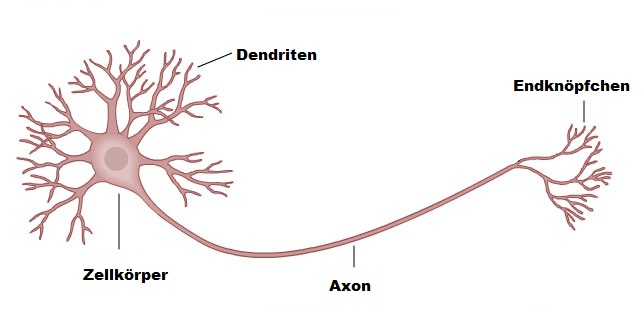
\includegraphics[width=0.7\textwidth, height=130px]{pics/neuron.jpg}	
	\caption{Schematische Darstellung eines biologischen Neuron \cite{bib:neuron}}
	\label{img:neuron}
\end{figure}
\begin{figure}
	\centering
	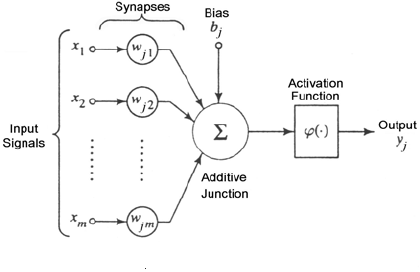
\includegraphics[width=0.7\textwidth, height=160px]{pics/aneuron.png}	
	\caption{Schematische Darstellung einer Möglichkeit, ein künstliches Neuron zu simulieren. Die Input Signale kommen von anderen Neuronen und werden gewichtet aufsummiert. Das Ergebnis der Aktivierungsfunktion wird als Output an andere Neuronen weitergeleitet. Mit dem biologischen Vorbild vergleichbar sind hier die Aufsummierung und Aktivierungsfunktion mit dem Zellkörper, die Input Signale mit den Gewichten mit Synapsen und der Output mit dem Axon.\cite{bib:aneuron}}
	\label{img:aneuron}
\end{figure}
\begin{figure}
	\centering
	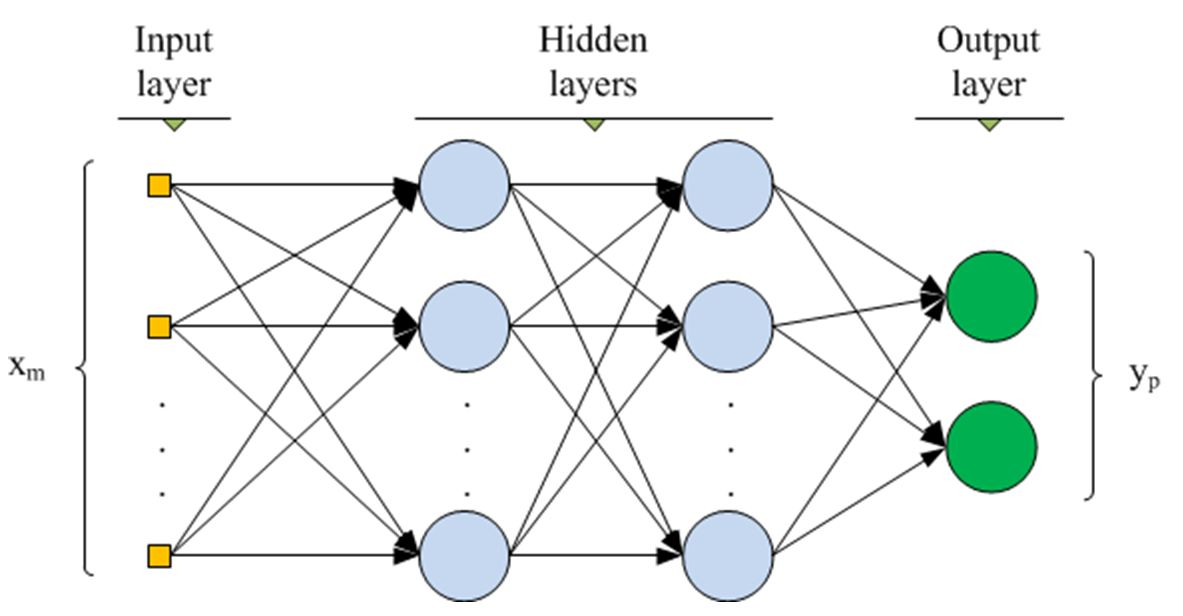
\includegraphics[width=0.7\textwidth, height=150px]{pics/mlp.jpg}	
	\caption{Ein Multilayer Perceptron mit m Inputneuronen(gelb), zwei Hidden Layern(blau) und zwei Outputneuronen(grün). Der Datenfluss ist in eine Richtung, Feedforward genannt.  \cite{bib:mlp}}
	\label{img:mlp}
\end{figure}
Es gibt viele verschiedene Arten von neuronalen Netzen, eine einfache von Ihnen ist das Multilayer Perceptron (MLP). Die Zellen werden zu mehreren Ebenen (Layer) zusammengefügt. Erst der Inputlayer, in das die Daten hineingegeben werden, dann die versteckten Layer, hier passieren die Berechnungen und werden dann an den Outputlayer weitergeleitet, aus welchem das Ergebnis des Netzes bezogen wird. Es gibt eine geordnete Datenflussrichtung Feedforward, eine Zelle erhält ihren Input von jeder Zelle der vorigenen Ebene und gibt ihren Output entsprechend an jede Zelle der folgenden Ebene weiter. Ein solches Netz sieht man in Abbildung \ref{img:mlp}.  
\begin{gather}
x_{j} = \varphi_{h}(net_{h}) = \varphi_{h}(\sum_{i=1}^{n} x_{i}w_{ij}) 
\label{eq:act}
\end{gather}
Wie man in Abbildung \ref{img:aneuron} sieht werden in jeder Zelle \(j\) die Inputsignale \(x_{i}\), also die Aktivierungen der vorigen Zellen mit Index \(i\) unterschiedlich gewichtet \(w_{ij}\)  und aufsummiert \(net_{h}\). Außerdem kann man den Layern eine Bias-Unit $ b_{j} $ hinzufügen, ein konstanter Wert normalerweise 1, welcher auch gewichtet wird und so einen anpassbaren Schwellenwert bzw. eine Verschiebung der Aktivierungsfunktion in beide Richtungen ermöglicht. Eben diese Gewichte sind der Kern des maschinellen Lernens, da bei einmal geschickt gefundenen Gewichten, komplexe Aufgabenstellungen und Probleme mit (vergleichsweise) wenig Rechen- sowie Programmieraufwand gelößt werden können. Im Wesentlichen versucht ein MLP immer eine Funktion zu berechnen welches einen Inputvektor der Größe \(n\) auf einen Outputvektor der Größe \(m\) abbildet.
\begin{gather*}
f_{MLP}: R^n \to R^m 
\end{gather*}
Ein Beispiel für eine solche Funktion wäre für ein gegebenes Bild zu entscheiden, ob darauf ein Gesicht zu erkennen ist. Die Länge des Inputs wäre hier z. B. mehrere hundert, die Pixelwerte bzw. daraus extrahierte Features eingesetzt, als Output wäre hier nur eine Zahl, nämlich ob ein Gesicht zu sehen ist oder nicht. Der Output \(y\) des Netzes ist also abhängig vom Input \(x\), aber auch von den Gewichten \(w\).
Die Gewichte werden entweder mit Hilfe von Trainingsdaten \textit{T}, bestehend aus Inputdaten und entsprechenden Outputdaten, also den zugehören Lösungen, oder mit einer zu erlenenden Zielfunktion, die einem aus gegebenen Inputdaten die gewünschten Lösungen liefert, über mehrere Trainingsläufe (Epochen) justiert. Fügt man in die Inputebene entsprechende Inputdaten \(x\) ein, berechnet die Aktivierungen aller Zellen, vergleicht die Aktivierungen \(y\) des Outputlayers des Netzes mit den gegebenen Lösungen \(z\) und erhält einen Fehler \( E(z,y)\): 
\begin{equation}
E(z,y) =_{def} \dfrac{1}{2} \sum_{i=1}^{m}(z_{i}-y_{i})^{2}	
\end{equation}
Die Herausforderung ist es nun, diejenigen Gewichte \(w\) zu finden, für die der Fehler über alle Trainingsdaten minimal ist.
\begin{equation}
arg_{w} min( \sum_{(x,z)\in T} E(z,f_{MLP}(w,x)))
\end{equation}
Bei der Anpassung der Gewichte der versteckten Zellen hat man aber das Problem, dass man keinen direkten Fehler für sie kennt, da man nur für die Outputschicht den gewünschten Output hat und so einen Fehler ermitteln kann. Als Lösung ist hier der Backpropagation-Algorithmus geläufig. Dieser besteht aus 3 Schritten, die entweder solang durchlaufen werden bis der Fehler einen festgesetzten Schwellenwert (Threshold) unterschreitet, oder eine vorgegebene Anzahl an Epochen durchlaufen wurde. 
\begin{description}	\item[Feedforward]\hfill \\
	Der Inputlayer wird mit der Eingabe des jeweiligen Testsatzes befüllt und die Aktivierungen vorwärts Layer für Layer, Zelle für Zelle berechnet.  
	\item[Backward-Pass]\hfill \\ 
	Das Ergebnis am Outputlayer wird mit der gewünschten Lösung des Testsatzes verglichen und der Fehler berechnet. Diese werden entsprechend gewichtet die unteren Layer rückwärts Zelle für Zelle rückpropagiert.
	\item[Anpassen der Gewichte]\hfill \\ Dies ist der wichtige Schritt, hier werden nun Zelle für Zelle die Gewichte entsprechend des Gradienten angepasst. Mit den neuen Gewichten ist in der Regel der Output des Netzes genauer, der Fehler also geringer und der Algorithmus lässt die Fehlerfunktion im Idealfall gegen 0 konvergieren. \cite{bib:aneuron}
\end{description}
Die Gewichte werden anhand des absteigenden Gradienten der Fehlerfunktion aktualisiert.  Hierzu werden \(\delta\)-Werte, die zur Berechnung der Gewichtsupdates nötig sind, wie folgt berechnet: 
\begin{gather}
\delta_{k} = \varphi_{k}'(net_{k})(x_{k}-z_{k}) \\
\delta_{h} = \varphi_{h}'(net_{h})\sum_{k\in K}w_{hk}\delta_{k} 
\end{gather}

Wobei erst nach der oberen Gleichung für die Outputlayer die \(\delta_{k}\) gebildet und in die jeweils unteren Layer nach der unteren Gleichung beim bilden der \(\delta_{h}\) gewichtet aufsummiert werden (Backpropagation). \textit{K} sind hier die Neuronen aus dem jeweils oberen Layer. Die Formel für das Gewichtsupdate mit einer Lernrate \(\eta\) lautet dann:
\begin{gather}	
	\Delta w_{ij} =_{def}  -\eta \frac{\partial E}{\partial w_{ij}} = -\eta x_{i}\delta_{j}  
\end{gather} 
Die Lernrate gehört zum stochastischen Gradientenabstieg (SGD) \cite{bib:sgd}. Sie verhindert zu große Gewichtsänderungen auf einmal, damit Optima nicht übersprungen werden und nicht zu große Schritte in falsche Richtungen gemacht werden. Mit einer Momentumrate $ \mu$ kann das lernen beschleunigt werden:
\begin{gather}	
\Delta w^{t} =  -\eta \nabla_{w^{t}}E + \mu \Delta w^{t-1}
\end{gather} 
Es gibt verschiedene Methoden SGD weiter zu optimieren, die von uns in dieser Arbeit verwendete ist die Adaptive Moment Estimation Methode (ADAM) \cite{bib:adam}. Sie kommt noch schneller zu genaueren Ergebnissen, indem sie die Momentumrate während des Trainings anpasst. Hierzu werden Parameter mit den Standardwerten $ \beta_{1}=0.9, \beta_{2}=0.99 $ und $ \epsilon = 10^{-8}$ eingeführt. Wobei $ \beta_{1} $ und $ \beta_{2} $ die Abklingraten des Einflusses der vergangenen Momenta auf den jetzigen Zeitschritt sind. Sind sie Nahe 1, klingt der Einfluss langsamer ab. $ \epsilon$ ist ein glättender Term, der Division durch 0 verhindert.

\section{Rekurrente Neuronale Netze}

Neuronale Netzwerke haben einen für einen 1-dimensionalen Inputvektor einen eindeutig zu berechnenden 1-dimensionalen Outputvektor und für die meisten Problemstellungen ist auch genau diese Kompetenz gefordert. Es gibt aber auch Probleme, bei denen der Output nicht nur von diesem, sondern auch von allen beziehungsweise einigen vorigen Inputs und Zuständen abhängt. Ein anschauliches Beispiel wäre hier die Klassifizierung von Videoausschnitten, wo die Bedeutung eines einzelnen Frames vom Kontext der vorigen Frames abhängt. Hingegen ein einfacheres Beispiel wäre das in dieser Arbeit betrachtete Bouncing Ball Szenario. Befindet sich ein Ball im Punkt \(p_{1}=(0/0)\) und der nächste Ort \(p_{2}\) soll vorhergesagt werden, ist es natürlich entscheidend ob der Ball sich zuvor beispielsweise im Punkt \(p_{0}=(0.1/0,1)\) oder im Punkt \(p_{0}=(-0.1/-0.1)\) befand. Hierzu werden den Zellen aus dem verstecktem Layer des neuronalen Netzes rekurrente (lat. recurrere: zurücklaufen) Verbindungen hinzugefügt.
\begin{figure}
	\centering
	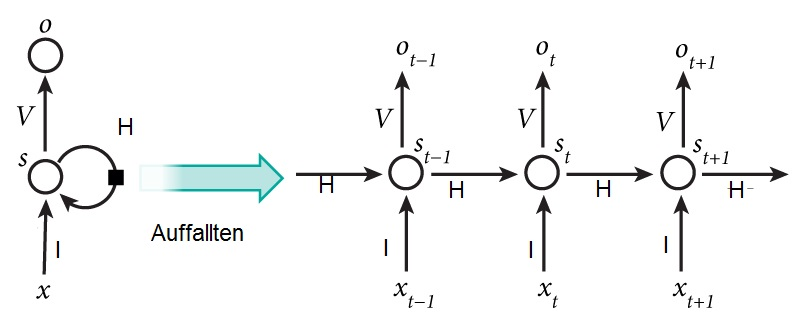
\includegraphics[width=0.7\textwidth, height=130px]{pics/rnn.jpg}	
	\caption{Um Backpropagation für ein rekurrentes Netz zu benutzen, muss man es durch die Zeit auffalten. \cite{bib:rnn}}
	\label{img:rnn}
\end{figure}
Eine Zelle \textit{h} bekommt nun im Zeitpunkt \textit{t} seinen Input immer noch von allen Zellen des unteren Layers \textit{I}. Zusätzlich nimmt sie aber auch noch als Input den Output aller Zellen desselben Layers, aber aus dem vorigen Zeitschritt \textit{H'}.Die Formel für die Aktivierung lautet also: 
\begin{gather}
x^{t}_{h}=\varphi_{h}(net_{h}^{t})=\varphi_{h}(\sum_{i \in I}w_{ih}x^{t}_{i}+\sum_{i \in H'}w_{h'h}x^{t-1}_{h'})
\end{gather}

Da diese neuen rekurrenten Inputs auch wieder gewichtet verarbeitet werden, müssen diese erst noch geschickt gefunden werden. Dies macht man mit Backpropagation durch die Zeit (BPTT) \cite{bib:bptt}. Dies passiert analog zur Backpropagation im MLP, jedoch werden die einzelnen Zeitschritte aufgeklappt (Abbildung \ref{img:rnn}). BPTT berechnet sich also wie folgt:
\begin{gather}
	\delta_{k}^{t} = \varphi_{k}'(net_{k}^{t})(x_{k}^{t}-z^{t}_{k}) \\
	\delta_{h}^{t} = \varphi_{h}'(net_{h}^{t})(\sum_{k \in K}w_{hk}\delta^{t}_{k}+\sum_{h' \in H'}w_{hh'}\delta^{t+1}_{h'})
\end{gather}

Wobei hier die obere Formel für die $ \delta $ jedes Neuron des Outputlayers und die untere für die Hiddenlayer berechnet. Für das Gewichtsupdate werden die Deltas noch über den betrachteten Zeitraum aufsummiert und analog zum Multilayer Perzeptron berechnet. Der Backpropagation Algorithmus wird angewendet um das Netz zu trainieren und passende Gewichte, auch für die rekurrenten Verbindungen zu erhalten. Nun hat man ein Neuronales Netz mit einer Art Kurzzeitgedächtnis, welches beim Auswerten des Inputs die nahe Vergangenheit mit in Betracht zieht. Gibt es in der Anwendung aber tiefere Abhängigkeiten, wo ein vergangener Input einen Einfluss auf die fernere Zukunft hat, hat auch das RNN noch Schwierigkeiten:.
\section{Das Vanishing Gradient Problem}
\begin{figure}
	\centering
	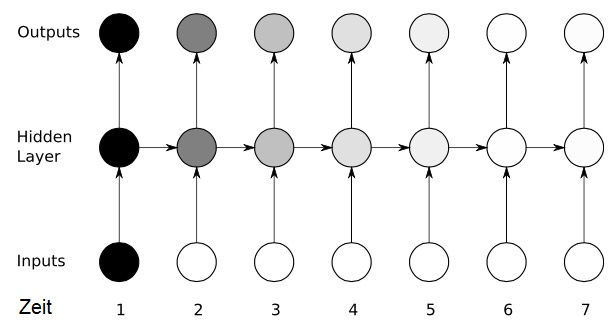
\includegraphics[width=0.7\textwidth, height=160px]{pics/vgp.jpg}	
	\caption{Das Problem vom verschwindenden Gradienten in einem rekurrenten Netz. Ein Fehler im Zeitschritt 1 erzeugt einen Gradienten, der aber auf die folgenden Zeitschritte immer weniger Einfluss hat.\cite{bib:graves}}
	\label{img:vgp}
\end{figure}
Wir haben gesehen wie beim Training eines rekurrenten Netzes über die Bildung des Gradienten Gewichte gefunden werden, die Probleme lösen können, bei denen Abhängigkeiten über die Zeit auftreten. Erstrecken sich diese Abhängigkeiten aber über zu große Zeitraume, tritt das Problem vom verschwindendem Gradienten (VGP) auf \cite{bib:vgp}. Mit den üblichen Aktivierungsfunktionen wie z. B der \textit{tanh}-Funktion treten Gradienten mit Betrag \(\leq\) 1 auf, bei der \textit{sigmoid}-Funktion sogar \(\leq 0.25\), die bei Backpropagation per Kettenregel miteinander multipliziert werden. Wird nun im Frontlayer ein Gradient berechnet, werden für \textit{n}-Layer im Netz, also auch für ein rekurrentes Netz das um \textit{n} Zeitschritte aufgefaltet wird, \textit{n} dieser kleinen Zahlen miteinander multipliziert, wodurch der Gradient exponentiell schnell sinkt. Hat man hingegen eine Aktivierungsfunktionen mit Gradienten Betrag \(\geq 1\), wächst der Gradient exponentiell schnell. Dies wird als Exploding Gradient Problem bezeichnet, das Pendant zum VGP \cite{bib:egp}.

Es bleibt aber zu erwähnen, dass dieses Problem nur beim automatisierten Training eines rekurrenten Netzes auftritt. Wenn man die Gewichte vorgibt und Aktivierungsfunktionen passend wählt, kann ein rekurrentes Netz Zellen als Speicherzellen verwenden. Z B. indem es immer den Wert, den es im letzten Zeitschritt als Output hatte, als Input nimmt, indem man dem rekurrenten Gewicht zur eigenen Zelle den Wert 1 gibt. Sinnvoll ist die Speicherzelle natürlich nur, wenn sie auch durch sogenannte Gate Zellen befüllt werden kann. Eine Input-Gate Zelle, welche reguliert ob, und mit was die Speicherzelle befüllt wird, eine Forget-Gate Zelle, welche die Speicherzelle wieder leeren kann und auch eine Output-Gate Zelle, die steuert ob die Speicherzelle ihren Inhalt ausgibt. Dies sind Strukturen die mit rekurrenten Neuronalen Netzen möglich sind und im kleinen Maß auch einfach zu erzeugen, wenn man die Gewichte manuell auswählen würde. Praktisch ist ein Neuronales Netz aber natürlich nur, wenn die Gewichte automatisch durch Training gefunden werden, dass solche Strukturen aber zufällig erzeugt werden, ist aber mit den bisher bekannten Trainingsmethoden quasi unmöglich. Wenn man jedoch eine Struktur fest vorgibt, funktioniert das Training und das Vanishing Gradient Problem wird überwunden. Eine mögliche solche Struktur sind die LSTM Zellen. 
\section{LSTM}
\begin{figure}
	\centering
	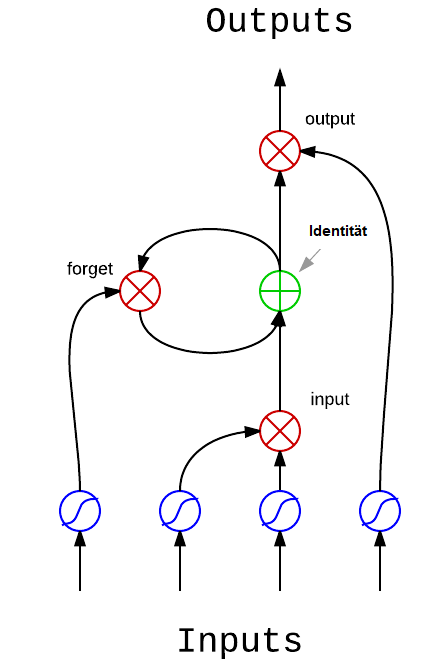
\includegraphics[width=0.5\textwidth, height=300px]{pics/lstm.png}	
	\caption{Ein Aufbau einer LSTM-Speicherzelle. 4 Neuronen (blau), die die 3 multiplikativen Gates lenken (rot), die das Verhalten der Speicherzelle steuern. Im inneren wird der Inhalt auf sich selbst abgebildet und mit neuem Input per Addition ergänzt (grün).    \cite{bib:lstmpic}}
	\label{img:lstm}
\end{figure}
LSTM steht für Long Short-Term Memory, also langes Kurzzeitgedächtnis. LSTM ist eine Struktur die man in rekurrente neuronale Netze einbaut um Speicherzellen zu erhalten, die Werte stabil über beliebig viele Zeitschritte speichern können. Üblich ist hierfür ein Aufbau wie in Abbildung \ref{img:lstm}. 4 Neuronen mit rekurrenten Verbindungen steuern das Verhalten der Speicherzelle. Eines steuert das Forget-Gate, also ob die Speicherzelle ihren gespeicherten Wert behalten soll. Im Normalzustand hat das Forget-Gate den Wert 1, sodass der gespeicherte Wert multipliziert mit 1 der Wert selbst bleibt. Soll ein Wert vergessen, bzw. nichts gespeichert werden, muss das Forget-Gate den Wert 0 annehmen. 2 Zellen steuern das Input-Gate, eine gibt den Wert an, welcher gespeichert werden soll und die andere steuert mit einem Wert zwischen 0 und 1, ob die Zelle einen neuen Wert speichert. Es gibt Varianten, wo das Input- und das Forget-Gate gekoppelt sind, sodass immer wenn ein neuer Wert gespeichert werden soll der alte gelöscht wird und umgekehrt\cite{bib:lstm3}. Ist dies nicht der Fall, wird das Ergebnis des Input-Gates auf den bisher gespeicherten Wert aufaddiert. Die 4. Zelle steuert das Output-Gate, interagiert also nicht mit dem Wert der Speicherzelle selbst, aber regelt, ob das Gespeicherte ausgegeben wird oder nicht. \cite{bib:lstm}
In einer Variation werden den Speicherzellen noch Peepholes hinzugefügt \cite{bib:peep}. Diese sind direkte Verbindungen vom inneren der Zelle zu den Neuronen , welche die Gates ansteuern. Dies hat den Effekt das die Gates den Inhalt ihrer Zelle auch dann kennen, wenn das Output-Gate geschlossen ist.  

In Abbildung \ref{img:lstm2} sieht man, wie der Inhalt der Speicherzellen sauber durch die Gates gelenkt werden kann. Das funktioniert im Forwardpass, aber auch genauso beim Training im Backwardpass mit dem Gradienten, da der Inhalt der Zelle per Identitätsfunktion durch die Zeit auf sich selbst abgebildet wird, und da der Gradient der Identität den Betrag \( = 1 \) hat, geht jetzt auch nichts mehr verloren. \cite{bib:lstm}. LSTM Netze werden wie rekurrente Netze mit BPTT trainiert.
\begin{figure}
	\centering
	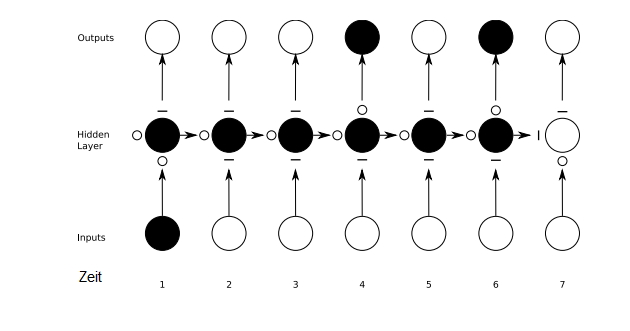
\includegraphics[width=0.7\textwidth, height=160px]{pics/lstm2.png}	
	\caption{Der Inhalt der Zelle wird durch die verschiedenen Zeitschritte durch die Gates gelenkt. Kreis bedeutet ein offenes Gate, ein Querstrich stellt ein geschlossenes Gate dar.    \cite{bib:graves}}
	\label{img:lstm2}
\end{figure}

LSTM wird in aktuellen Produkten von bedeutenden Technologie Firmen wie zum Beispiel Apple\cite{bib:apple}, Amazon\cite{bib:amazon} und Google als Kernkomponente verwendet. Von Google zum Beispiel für die Spracherkennung für den Smartphoneassistenten Allo\cite{bib:allo}. 

Nun wollen wir in dieser Arbeit untersuchen, wie das LSTM in seinen Zellen mit Events umgeht. Für die Unterteilung durch Events gibt es aus der Psychologie bereits einen Ansatz, die Event Segmantation Theory (EST).

\section{Event Segmentation Theory}
Ein Weg etwas zu verstehen, ist es in kleinere Teile zu Unterteilen. Nach der Event Segmentation Theory (EST) \cite{bib:est1} ist das Unterteilen von kontinuierlicher Aktivität durch bedeutungsvolle Ereignisse eine Kernkomponente der Wahrnehmung.  Dies ist sowohl ein Top-Down also auch ein Bottom-Up Vorgang, also sowohl das Wissen über die Pläne des beobachteten Akteurs als auch der direkte sensorische Input haben Einfluss auf diese Unterteilung.\cite{bib:est} Die Planung zum Erreichen eines Ziels ist in Events unterteilt. Z. B. wenn man jemandem zuschaut wie er sein Zelt aufbaut, erwartet man, wenn man den Vorgang kennt, dass dieser erst das Zelt aus der Verpackung holt, das Zelt ausbreitet, die Stangen zusammensteckt, usw.. Diese Unterteilung ist für uns ganz natürlich und dazu macht es keinen Unterschied, ob man sich zum Zusammenstecken der Stangen z. B. auf den Boden setzt, auch wenn das physisch ein ganz anderer Vorgang ist. Die Bottom-Up Seite von EST greift auf ein Model zurück, bei dem das Gehirn ständig Vorhersagen über die Umwelt macht und resultierende entdeckte Fehler verarbeitet \cite{bib:est}. Befindet sich der beobachtete Akteur in einem Event, werden sich dessen folgenden Bewegungen und Aktionen stetig an seine vergangenen Aktionen anschließen. Hat man hingegen eine hohe Unsicherheit in der Vorhersage der nächsten Aktionen, wird eine Ereignisunterteilung vorgenommen. Am Beispiel: Ist jemand gerade beschäftigt mit dem zusammenstecken der Zeltstangen, wird er das erfahrungsgemäß auch weiterhin machen, ist er damit aber fertig, ist unklar ob er z. B. erst das Vorzelt aufbaut, uns als Beobachter um Hilfe bittet oder sich erstmal einen Kaffee holt, welche auch unterschiedliche Aktionen unsererseits fordern würden.
Entgegen dem alltäglichen Sprachgebrauch meint EST mit Ereignissen immer ganze Vorgänge, also z. B. das Zusammenstecken der Zeltstangen, nicht aber das Beginnen oder das Fertigwerden, diese werden als Ereignisgrenzen bezeichnet. Ereignisse sind verschieden granuliert und hierarchisch, so ist z. B. das Zusammenstecken der Zeltstangen Teil des Ereignisses des Aufbauen des Zeltes, welches wiederum Teil des Ereignisses Campingurlaub ist.

In Abbildung \ref{img:est} sieht man, wie eine Unterteilung nach Bedeutung dem Verstehen hilft. EST sieht seine Gültigkeit sowohl beim beurteilen und vorhersagen der Aktionen anderer, als auch beim Durchführen und Planen der eigenen.


\begin{figure}
	\centering
	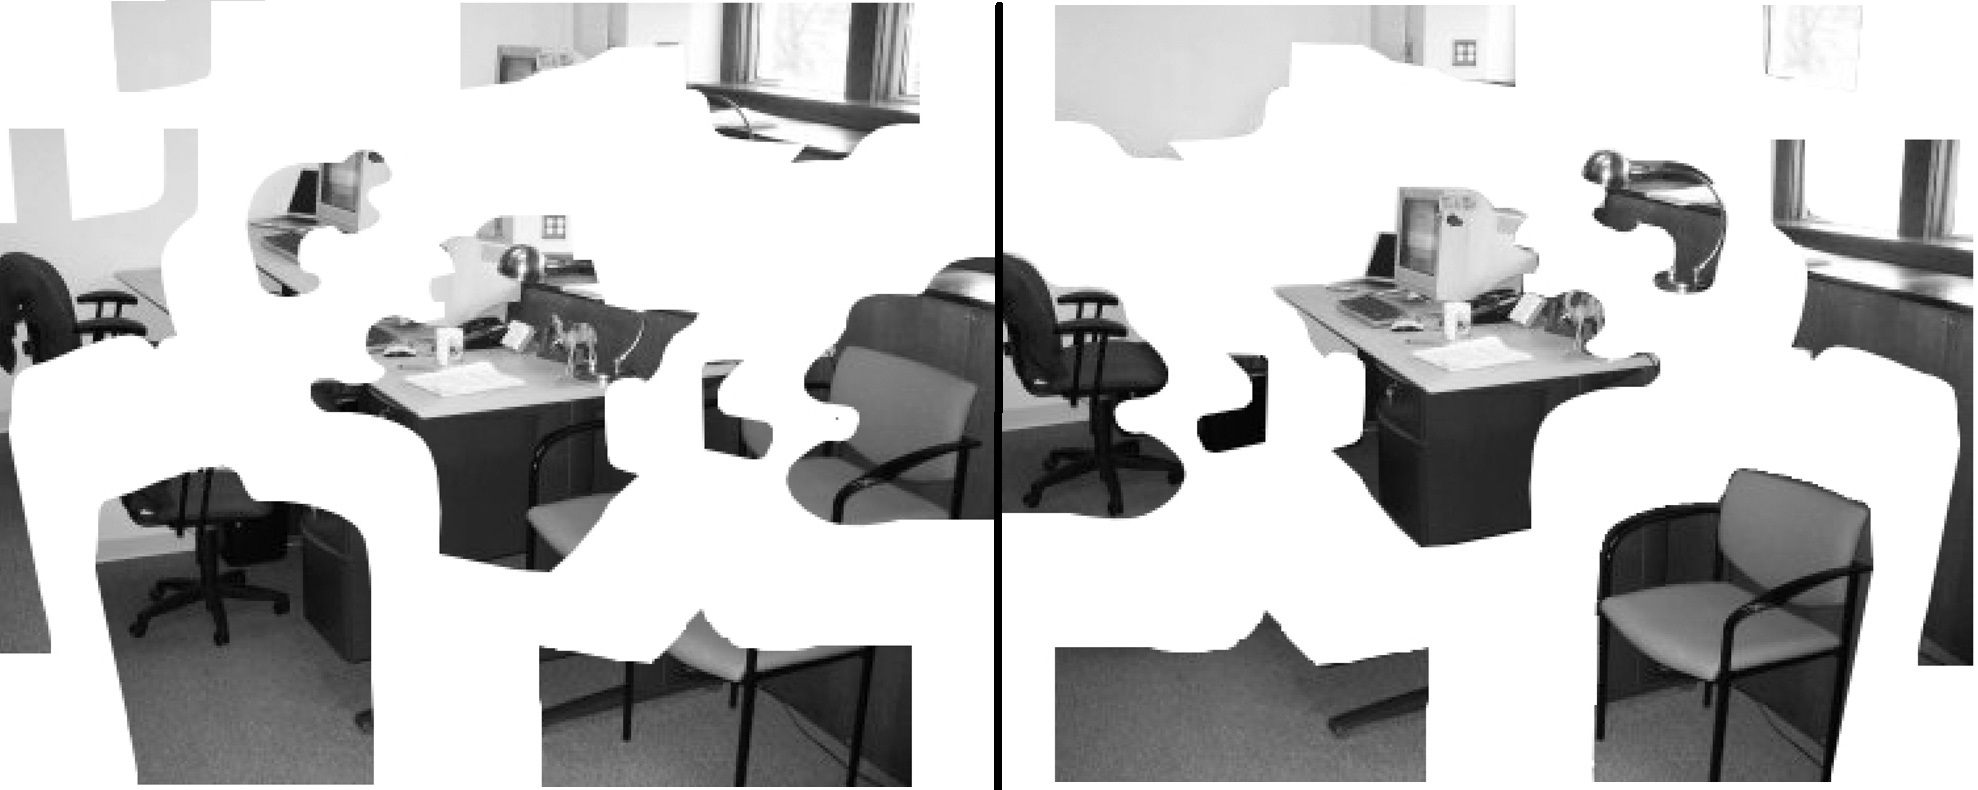
\includegraphics[width=0.9\textwidth, height=130px]{pics/est.jpg}	
	\caption{Ein Bild einer Büroszene in 2 verschiedenen Weisen zerschnitten. Für die linke Version benötigt man mehr Anstrengung, um die Szene zu verstehen. Es veranschaulicht, wie eine Zerteilung nach Bedeutung die Wahrnehmung unterstützt. \cite{bib:est}}
	\label{img:est}
\end{figure}


\chapter{Implementation}
Nun da die Grundlagen gelegt sind können wir anfangen zu untersuchen wie ein LSTM Netz mit Events umgeht. Wir betrachten dazu das Bouncing Ball Szenario, da es klare Events hat und sich dadurch auch gut segmentieren lässt. Zur Implementation wurde JANNLab (Otte et al. 2013), ein Java Framework für Neuronale Netze verwendet \cite{bib:jannlab}. Dieses Kapitel soll die im Zuge dieser Arbeit verwendeten Techniken erklären und aufzeigen wie die im nächsten Kapitel beschriebenen Ergebnisse erreicht wurden, sowie welche Probleme sich dabei in den Weg gestellt haben.

\section{Das Bouncing Ball Szenario}
Das Bouncing Ball Szenario beschreibt einen Ball, der gleichförmig durch die Ebene gleitet bis er an entsprechenden Begrenzungen abprallt. Wir haben die 1- und die 2-dimensionale Version verwendet.

Im 1-D Fall haben wir einen Ball ohne Ausdehnung (also eigentlich ein Punkt aber diese Unterscheidung ist für unsere Zwecke irrelevant) mit einer Position $ x_{b} $ und einer konstanten Geschwindigkeit $  v$. Dieser springt zwischen den Grenzen $ x_{1}=-1 $ und $ x_{2}=1 $ hin und her, also immer wenn die Position des Balls eine der Grenzen annimmt, wird die Geschwindigkeit invertiert $ v := -v $. Also genau so wie man es sich vorstellt.

Der 2D Fall funktioniert analog, der Ball hat eine Position $ (x_{b}/y_{b}) $, eine konstante Geschwindigkeit $ (v_{x}/v_{y}) $, welcher nun zwischen den 4 Grenzen $ x_{1}=-1 $ und $ x_{2}=1 $, $ y_{1}=-1 $ und $ y_{2}=1 $ hin und her springt. Nimmt nun eine Koordinate des Balls eine der Grenzen an wird die entsprechende Koordinate invertiert, also $ (v_{x}/v_{y}) = (-v_{x}/v_{y}) $ beziehungsweise $ (v_{x}/-v_{y}) $. 

Das 1D-Szenario habe ich hauptsächlich verwendet um mich einzuarbeiten und zurechtzufinden, da es unter anderem mit weniger Neuronen erlernt werden kann und so die Aktivierungen der einzelnen Gates auch übersichtlicher sind. Der Grund warum das 1D-Szenario auch für diese Ausarbeitung wichtig ist, ist das unter Hinzunahme der Zeitachse aussagekräftige Diagramme erstellt werden können, anhand derer einige Trainingseffekte und Verläufe veranschaulicht werden können. Entsprechende Analysen konnten vom 2D-Fall auch gemacht werden, wenn man sah wie sich eine Linie oder ein Ball mit Verzögerung entsprechend über den Bildschirm bewegt, die resultierenden Bilder sind jedoch eher unübersichtlich. Das 2D Szenario hingegen ist das für unsere Untersuchungen interessantere, da es mehr Events gibt, die auch in komplexernen Beziehungen zueinander stehen. In Abbildung \ref{img:1dvs2d} sieht man jeweils 2 Beispiele, zu dem genauen Aufbau des dazu benutzten LSTM Netzes kommen wir in der folgenden Sektion.
\begin{figure}
	\centering
	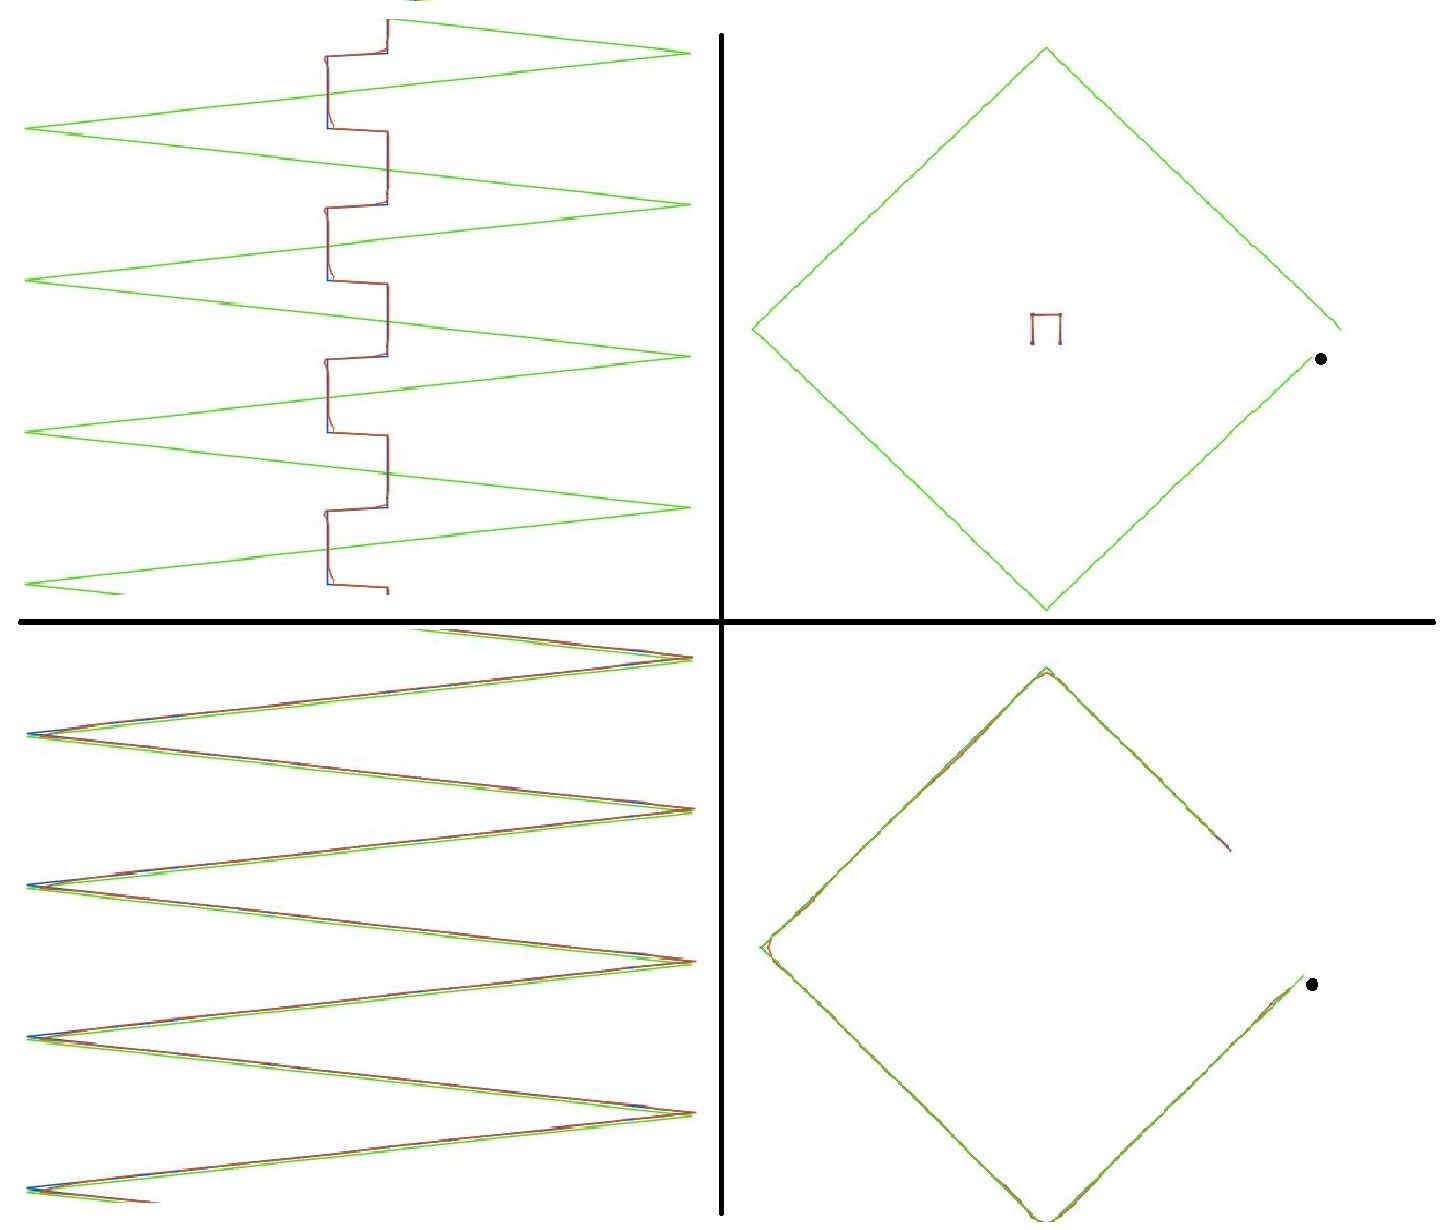
\includegraphics[width=0.9\textwidth, height=370px]{pics/1dvs2d.jpg}	
	\caption{4 Versionen des Bouncing Ball Szenario erlernt durch LSTM Netze. Zu sehen sind der Netzinput (grün), der Netzoutput (rot) und das Trainingsziel (blau). Links sieht man 2 Beispiele des 1D Falls, zur besseren Veranschaulichung sind die Daten nach den Zeitschritten vertikal versetzt. Rechts sieht man 2 Beispiele des 2D Falls, die Abbildung zeigt jeweils den Verlauf des Balls bis kurz vor dem vollenden einer Runde, um Überlagerungen in der Abbildung zu vermeiden. Der Startpunkt ist durch den schwarzen Punkt gekennzeichnet. In den jeweils oberen Fällen wurde als Netzinput die Position des Balles und als Trainingsziel die Geschwindigkeit des Balles für den nächsten Schritt. In den jeweils unteren Fällen wurde als Netzinput die Position des Balles und als Trainingsziel die vorauszuberechnende nächste Position des Balles.}
	\label{img:1dvs2d}
\end{figure}

\section{Unser LSTM, Parameter + Testfälle}
Für unser LSTM-Netz haben sich folgende Parameter als sinnvoll erwiesen:
\begin{description}	\item[Aktivierungsfunktionen:]\hfill \\ 
	Zur Ansteuerung der Gates der LSTM-Zellen im Hiddenlayer werden Neuronen mit \textit{Tangens hyperbolicus} als Aktivierungsfunktion verwendet. Für das Outputlayer wird zur Aktivierung die lineare Funktion verwendet, da die Position des Balles gleichverteilt Werte zwischen -1 und 1 annimmt, soll unser Netzoutput dasselbe tun. Anfangs war für das Outputlayer per Defaultoption die \textit{sigmoid}-Funktion zur Aktivierung eingestellt, deren Bild aber nur von 0 bis 1 reicht. Das hatte natürlich nicht funktioniert und für Verwirrung gesorgt, warum denn nur die Hälfte des Problems erlernt wird.  
	\item[Trainingsoptimierung:]\hfill \\ 
	Als Optimierungsmethode für das Traing wurde die Adaptive Moment Estimation Methode(ADAM), also eine adaptive Momentumsschätzung, verwendet. Diese baut die übliche Lernmethode mit Lernrate und Momentumrate dahingehend aus, dass diese durchgehend angepasst werden, um noch schneller zu genaueren Ergebnissen zu kommen. Hierzu wurden die Standard Parameter verwendet, also $ \beta_{1}=0.9, \beta_{2}=0.99 $ und $ \epsilon = 10^{-8}$. Wobei $ \beta_{1} $ und $ \beta_{2} $ die Abklingraten des Einflusses der vergangenen Momenti auf den jetztigen Zeitschritt sind. Sind sie Nahe 1, klingt der Einfluss langsamer ab. $ \epsilon$ ist ein glättender Term, der Division durch 0 verhindert. \cite{bib:adam} Es wurde für Debugging-Zwecke an diesen Werten herumgespielt, es wurden aber nie sichtlich bessere Ergebnisse erzielt.
	\item[Netzgröße:]\hfill \\ 
	Die passende Netzgröße ist  fallabhängig, in Abbildung \ref{img:1dvs2d} wurden für die 1D Fälle 1-2-1 Netze verwindet (also 1 Inputneuron, 1 Hiddenlayer mit 2 Neuronen und 1 Outputneuron), für die 2D Fälle 2-4-2 Netze. An anderer Stelle werden andere Netzgrößen verwendet, dann wird das an entsprechender Stelle auch nochmal aufgegriffen.
	\item[Außerdem:]\hfill \\
	Alle Layer sind mit Bias-Unit, um mit möglichst wenig Neuronen möglichst viel Funktionalität zu erreichen, damit deren Analyse wiederrum möglichst ausgiebig verläuft. Peepholes \cite{bib:lstm2} wurden getestet, hatten in diesem Beispiel keinen sichtbaren Effekt auf das Training und wurden dann weggelassen.  
\end{description}
Außerdem wurden verschiedene Testfälle mit verschiedenen Intentionen betrachtet, die ich aber an dieser Stelle vorgreifend definieren möchte:
\begin{description}
	\item[Verschiedene Inputs:]\hfill \\
	
	\item[Verschiedene Outputs:]\hfill \\
	
	\item[Zufällige Startposition + Geschwindigkeit:]\hfill \\
	
	\item[Feedback:]\hfill \\
\end{description}


\section{Das Training des Bouncing Verhaltens}

\section{Umfragen zum Thema}
1 von 1 befragten Personen mit einem Abschluss in Bachelor of Science meinten zum Thema: \\
Davon weiß ich nichts. \cite{bib:lstm}


\section{Feedback}



Das Training des Bouncing Verhaltens
Das interessante am Bouncing Ball Szenario ist natürlich nicht die gleichförmige Bewegung, sondern das nicht-lineare Verhalten beim Abprallen. Dieses wollen wir unserem LSTM Netzwerk möglichst genau erlernen und haben dazu einige Techniken angewendet. 

Reaktives vs vorhersehendes Verhalten
1D mit 1b Zelle

RNN Annäherung vs echte nichtlinearität
Random vs nicht Random, nur periodisch gelernt
Feedback für random, erklären warum es nicht funkltioniert hat,
Feedback, Zittern erklären für Input außerhalb des eigenen Raums
Schritte damit es funktioniert, feedback annäherung, hat nicht geholfen
Random diskretisiert um numerisch genau definiertes Rand verhalten zu haben
\chapter{Gates und Eventgrenzen}
\label{ch:untersuchung}
Nun haben wir also Neuronale Netz mit LSTM Speicherzellen auf verschiedene Fälle des Bouncing Ball Szenarios trainiert. Wenn man dabei die internen Aktivierungen der Gates über die Zeit betrachtet und vergleicht mit dem Verlauf der Ereignisse der trainierten Aktion, findet man Zusammenhänge. In diesem Kapitel werden wie erst Beispiele für solche Zusammenhänge betrachten, dann schauen wie man diese automatisiert finden kann. Zum Schluss schauen wir noch, wie wir mit Hilfe von Backpropagation through time Vorhersagen über Events anhand der Gate-Aktivierungen treffen können und wir dieselbe Technik nutzen können um die Eventbeziehungen zu klassifizieren.
\section{Gate-Aktivierungen}
Die Möglichkeiten wie sich eine LSTM über die Zeit verhalten kann sind zahlreich, noch zahlreicher die Möglichkeiten wie mehrere von ihnen miteinander interagieren. 



\\ 
\begin{tabular}{|c|c|c||c|c|c|}
\multicolumn64}{|c|}{O = A+0.5B; P = B OR (1-C); Q = A XOR C} \\	\hline
A & B & C & O & P & Q \\ \hline
0 & 0 & 0 & 0 & 1 & 0\\ \hline
0 & 0 & 1 & 0 & 0 & 1\\ \hline
0 & 1 & 0 & 0.5 & 1 & 0\\ \hline
0 & 1 & 1 & 0.5 & 1 & 1\\ \hline
1 & 0 & 0 & 1   & 1 & 1\\ \hline
1 & 0 & 1 & 1   & 0 & 0\\ \hline
1 & 1 & 0 & 1.5 & 1 & 1\\ \hline
1 & 1 & 1 & 1.5 & 1 & 0\\ \hline \hline
\multicolumn{6}{|c|}{Backpropagation für O:=-1} \\ \hline
$\sum A $ & $\sum B $ &$\sum C $ & -1 & P & Q \\ \hline
2.64 & 1.35 & -1.5*$ 10^{-4} $ & -1 & P & Q \\ \hline
\multicolumn{6}{|c|}{Backpropagation für P:=-1} \\ \hline
$\sum A $ & $\sum B $ &$\sum C $ & O & -1 & Q \\ \hline
9*$ 10^{-4} $& 0.07 & -0.07 & O & -1 & Q \\ \hline
\multicolumn{6}{|c|}{Backpropagation für Q:=-1} \\ \hline
$\sum A $ & $\sum B $ &$\sum C $ & O & P & -1 \\ \hline
-0.81 & $ 10^{-3} $ & 0.81$ & O & P & -1 \\ \hline
\end{tabular}
\hline
 

\begin{figure}
	\centering
	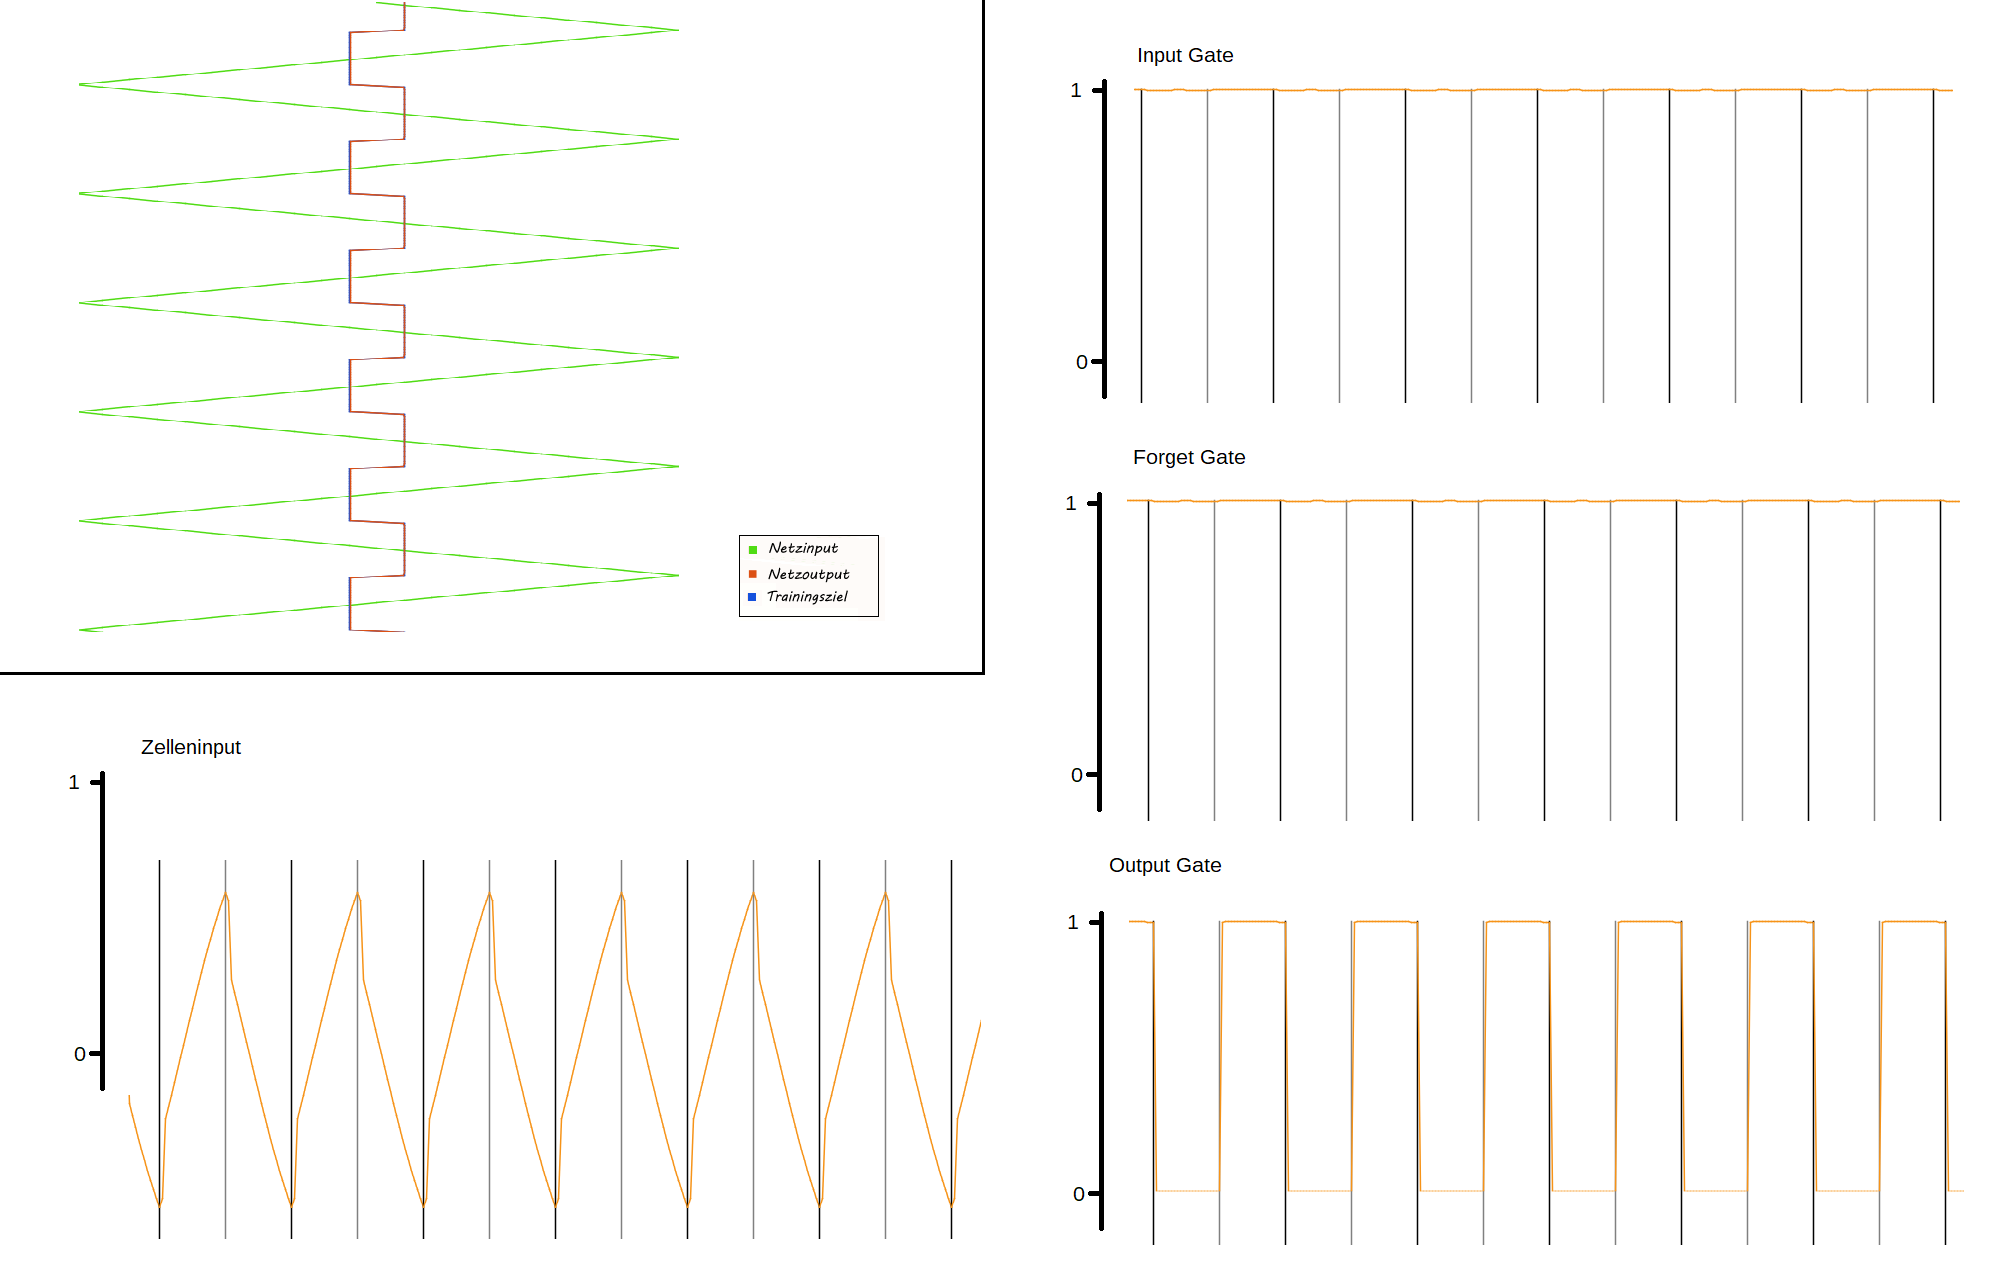
\includegraphics[width=0.9\textwidth, height=400px]{pics/act1.png}	
	\caption{Der 1D Fall mit Ballposition als Netzinput und nächste Geschwindigkeit als Trainingsziel, gelernt von einem 1-1-1 Netz.  }
	\label{img:act1}
\end{figure}


\cite{bib:graves}

\section{Automatisierte Klassifizierung}




\section{Analyse mit BPTT}

periodisch: sieht man immer, das nicht das problem, sogar klar. overfitting

Verhalten an der Eventgrenze:

runde annäherung nicht erwünscht, aber wird es immer sein nur eben immer unrunder. im besten fall, dauert die eventgrenze immernoch über 4 zeitschritte an(1D-Fall), was durch Diskretisierung abgehackt aussieht, aber doch eine kurve ist bei kontinuierlich




RNN Annäherung vs echte nichtlinearität

anders als angenommen: zufall war garnicht wichtig. Alles was bestätigt wurde, 2 1D Fälle überlagert

dieser fall den man bekommen hätte mit feedback und zufällig und perfekt trainiert, vllt sogar viel langweiliger, da event tatsächlich nur von position des Balles abhängt, nur ein einzelnes Gewicht, wenn 1 erreicht ausgelöst ohne interaktion. 


mit backpropagation im 1D fall, sieht man: Lstm zelle forgetgate ist auf 1. wir bewegen uns nach links. wenn man gradient +1 wählt, kommt dann auf selbe zelle negativer gradient zurück? also um wieder nach links zu gehen muss man erstmal nach rechts gehen. 

Wunschergebniss, falls man es nicht sieht beschriebe es un erzähle warum man es nicht sieht: 
Hat ein Netz ein Event gut gelernt, merkt man das auch anhand der Zellen die eventeinteilung klappt besser.
Dierekter zusammenhang: lstm netz gut trainiert, mlp zur est gibt gute ergebnisse.

Wunschergebniss
Unterschiede zwischen random und nicht random
Bei random funktioniert est viel besser,  da  durch unterschiedliche geschwindigkeiten die eventkanten besser gelernt werden müssen, bzw bei nicht random werden periodische funktionen gelernt die die event segmentation behindern.

Vergleiche: Testfälle Random 1 und Random 2 Richtungen. Inwiefern weisen die LSTM zellen hinweise auf eventsegmentation? 

Vergleiche: 2D mit 6-8 und 16 zellen gelernt.
Und mit 4? Was ist die kritische Zahl?

Erstelle eine Ansicht, die anzeigt welche Zellen und Werte genutzt wurden.

Stelle 2 Hypothesen auf was den in den Gates untersucht wird, ist es ob ich mich grad nach oben rechts bewege oder das oben und links die letzten Events stattgefunden haben.

Teste 2 verschiedene mlp formen: 4 outputs für wahrscheinlich des nächsten events,
oder 2 outputs für wahrscheinlich das jeweils konträre die nächsten sind.


Vorzeigefall: Rekurenz grundding: Gleicher Input kann abhängig von vorigen stats unterschiedlichen outputs leifern, man befindet sich dank lstm auch in unterschiedlichen gatepositionen.
Zeige ball der in 0,0 sitz der nach unten rechts un nach oben links fliegt und die aktivierungen

Feedback sollte integriert werden, um die eventtransition mehr zu werden. Darlegen warum event sauberer is wenn feedback benutzt ist. Vllt hätte das auch zu klareren events geführt. Für klarrerer events wurde auch neues random entwickeld bei dem die kante bei jedem step sauber getroffen wird.

Kann MLP abschätzen wie Nahe das Event ist?
Verschiedene Thresholds, Event in 2 Steps, 5 Steps, 10 Steps, Alarm geben wenn Kollision bevorsteht.

Erklären wie die Trainingsdaten für das mlp aussehen

Vergleiche mlp das next und last event sagt
Vorhersage: last event exakt deutlich, next event unklarer das ob oben oder rechts als nächstes getroffen wird vom vall abhängt wenn man von links unten kommt-

Wichtig:
Vergleiche im LSTM die bedeutung der einzelnen Gates auf EST. Zentral


%\chapter{Zusammenfassung und Ausblick} 
\label{ch:ende}
leer...
\section{Zusammenfassung}
leer...
\section{Ausblick}
leer...
%\chapter{Anhang} 
\label{ch:appendix}

\newpage


% Ab hier kommt der Anhang (optional)
%\appendix
%\input{chapters/11-appendix}

% Literaturverzeichnis
\cleardoublepage



\bibliographystyle{abbrv}
\bibliography{literature}


\end{document}

